\begin{figure}
  \centering
  \begin{subfigure}[htpb]{0.8\textwidth}
   \centering
   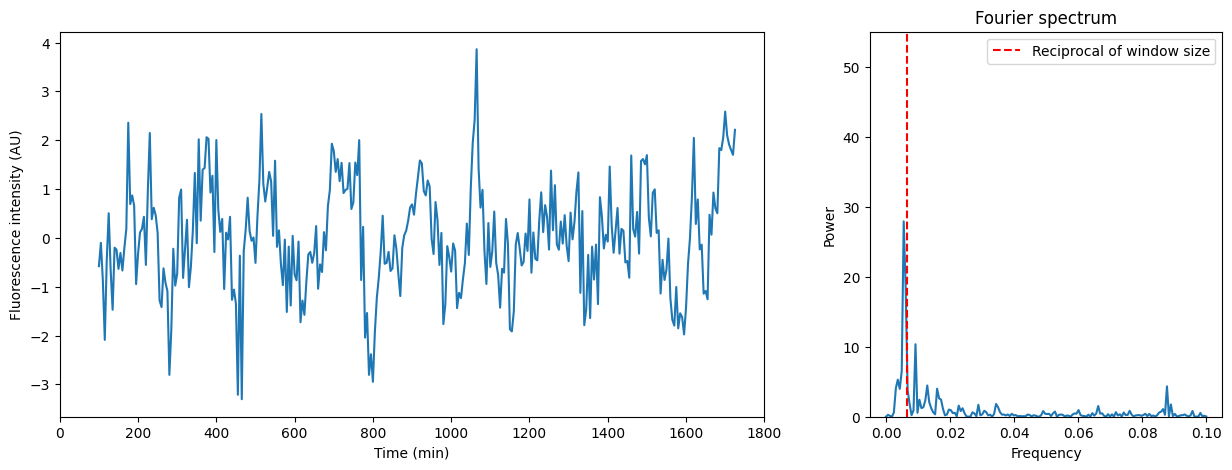
\includegraphics[width=\textwidth]{fft_slidingwindow}
   \caption{
   }
   \label{fig:analysis-slidingwindow-movavg}
  \end{subfigure}

  \begin{subfigure}[htpb]{0.8\textwidth}
   \centering
   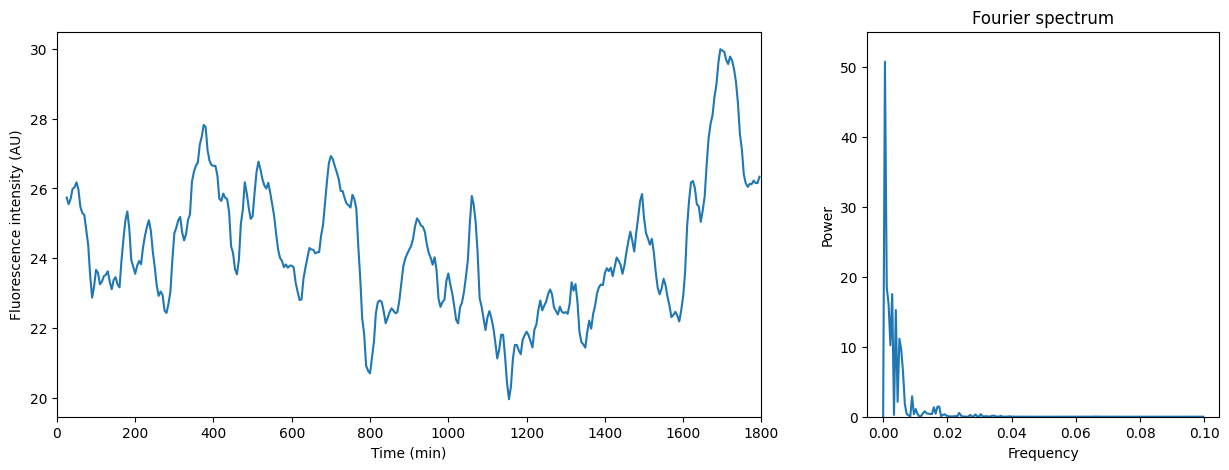
\includegraphics[width=\textwidth]{fft_savgol}
   \caption{
   }
   \label{fig:analysis-slidingwindow-savgol}
  \end{subfigure}

  \caption{
    (Left panels) Raw time series with trends, (middle panels) processed time series, and (right panels) Fourier spectra to demonstrate
    \textbf{(\ref{fig:analysis-slidingwindow-movavg})}
    using a moving average (window size 30), and
    \textbf{(\ref{fig:analysis-slidingwindow-savgol})}
    using a Savitzky-Golay filter (window size 7, polynomial order 3)
    to remove trends.
  }
  \label{fig:analysis-slidingwindow}
\end{figure}
